\documentclass[a4paper, 11pt]{report}
\usepackage[T1]{fontenc}
\usepackage[utf8]{inputenc}
\usepackage[english]{babel}
\usepackage{graphicx} % support graphics
\usepackage{hyperref} % links in the document
\usepackage{fullpage} % smaller margins
\usepackage{float} % position of figures
\usepackage{color}

% Define path where the plots are stored
% \def  \plotpath {../code/A/plots/}

% Use a new command to wrap std functionality
\newcommand{\insertplot}[3][H]{
	\begin{figure}[#1]
	    \begin{center}
	        \includegraphics[width=0.7\textwidth]{../code/A/plots/#2}
	    \end{center}
	    \caption{#3}
	    \label{fig:#2}
	\end{figure}
}

% Configure different colors
\definecolor{darkred}{rgb}{0.5,0,0}
\definecolor{darkgreen}{rgb}{0,0.5,0}
\definecolor{darkblue}{rgb}{0,0,0.5}

% Set hyperlink settings
\hypersetup{ 
	colorlinks = true, 
	linkcolor=darkblue, 
	filecolor=darkgreen, 
	urlcolor=darkred , 
	citecolor=darkblue 
}

\title{Project 1.A: \\ Programming the Basics of an \\ Evolutionary Algorithm(EA)}
\author{Mikael Brevik}
\date{\today}

\begin{document}
\maketitle
\tableofcontents


\chapter{Introduction}
\section{About the project}
The purpose with this project is to gain expirience with the basic mechanisms underlying EAs
by programming them.

The entire project consists of two parts; A) Implementing basic modular EA , and B) using that 
algorithm to solve a Colonel Blotto problem.  

This document will focus on part A, implementing the basic evolutionary algorithm and testing
that algorithm by solving a One Max problem

\section{EA Overview}
The evolutionary algorithm we're implementing in this assignment includes the following aspects:

\begin{enumerate}

	\item A population for reperesenting indeviduals with genotypes.
	
	\item A development phase, for converting genotypes to phenotypes.
	
	\item A fitness test for calculating fitness of all phenotypes.
	
	\item Selection protocols for finding adults from the indeviduals
	
	\item Selection mechanism for finding parents from the adults. 
	
	\item Reproduction for creating children from parents. Taking parts from each of the parent's genos. 
	
	\item Mutation for altering the childrens genotype. 

\end{enumerate}

\noindent{The EA will loop through these items many generations. There must also exist a plotting 
functionality for analyzing and visualizing the results.}

\section{The One-Max Problem}

For testing out the EA, the One-Max problem will be used. The goal of the One-Max problem is to find a 
bit string consisting only of 1's. The initial genotype will be a random n-bit string. With using the number
of 1's as fitness, throughout the generations the bit strings should evolve to consist only of 1's. 

The programmed EA should be able to solve a 40-bit One-Max problem. 

\chapter{Deliverables}	
\section{Description of the EA code}
\label{sec:desccode}
The code aims to be highly object oriented. With this comes many classes and subclasses. All of the different 
aspects of a EA is represented as classes. 

In this section, an explanation of all the different main classes could be found.

\subsection{Third party libraries \& Dependencies}
\label{sec:thirdparty}

This application is dependent on a third party module/library for plotting the data. The library used
is matplotlib. Matplotlib, in turn, is dependent on other libraries. Libraries required are therefor dependent
of what dependencies matplotlib have. Some of them are NumPy and SciPy. 

\subsection{Code Overview}

The main classes includes: Plotter, Reproduction, Mutation, Population, SelectionStrategy and EA.
There's also a main-module which ties this all together and executes the application. 

The EA class is the main class, all other elements are tied to this class. 

\begin{figure}[h!]
    \begin{center}
        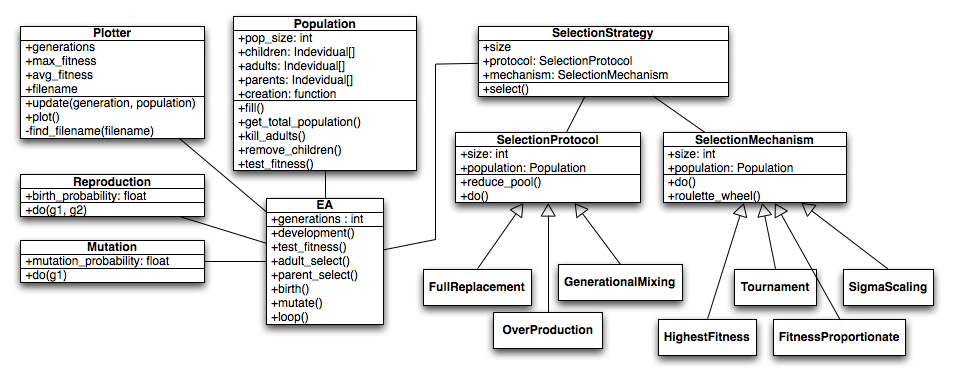
\includegraphics[width=\textwidth]{diagrams/classdiagram.png}
    \end{center}
    \label{fig:classdiagram}
    \caption[Class diagram]%
    {Class diagram for the basic EA. Not all subclasses and attributes of subclasses are included.}
\end{figure}

\subsection{Individual}
This is where the genotype, phenotype and fitness value gets stored. This class also have 
a method for calculating fitness value, based on a fitness function given as a parameter to
the constructor. You would normally inherit from this class in your EA.
The class also have an empty implementation of the function $create\_child$. This is used as an
abstract method. Subclasses should have their own implementation of the $create\_child$ method. \\


In the One-Max problem, this class gets extended to an BinaryVector class. This is a pretty shallow
extension. All it does is implement conversion between genotype and phenotype, create a randomly
chosen value representation and implement the $create\_child$ method.

\subsection{Population}
The Population class stores all information about all the individuals. It has separation for children and adults.
It also holds temporary information about the adults selected as parents. 

The population class has a method for looping through all individuals and calculate fitness using the individual's
fitness() method. If there's need for a free for all competition in the fitness testing (like in Colonel Blotto), the 
population class could be extended and the $test\_fitness()$ method can be overwritten. \\

The population class also holds a method for filling a population with individuals. This is used by sending a 
closure function as a constructor argument, and executing the $fill()$ method. A closure function is a function
storing values and returning a function that uses those stored values. This is used to make the filling of the
population as generic as possible. So typically, the returning function should return an instance of the Individual
class (or a subclass).

\subsection{Selection Strategy}
As seen in the \hyperref[fig:classdiagram]{class diagram}, the Selection Strategy consists of multiple classes
and subclasses. There are two classes in direct contact with the SelectionStrategy class; Protocol and Mechanism.
Those two classes, contain the implementation of the different protocols and mechanisms. Both have a similar
interface with the do method and a subclass for each different implementation.

In the do method, the population gets altered according to the rules specified by the protocol or strategy. The
main SelectionProtocol class, has a $reduce\_pool()$ method. This can be used by the protocols to reduce the 
population to a fitable size. I.e with ($\mu$, $\lambda$) and ($\mu + \lambda$) selection. \\

The mechanisms are slightly more complex than the protocols. With mechanisms using roulette wheel, the 
subclass need to override the probability function inherited from the base class. This method is used to find the
different "degree of sectors" on the roulette wheel. If the probability function uses aggregated values, such as
fitness sum, average fitness and so on, one could implement those in a $set\_values()$ method and set values
as object variables. Run the $set\_values()$ method in the $do()$ method. This way no unnecessary calculations
are performed. The mechanisms using roulette wheel should return the execution of the $roulette\_wheel()$
method.  \\

The SelectionStrategy class is an umbrella for protocols and mechanisms. Based on what constructor 
argument get's sent in. The arguments are one for protocol and one for mechanism. So if the FullReplacement
protocol is to be used, the argument will be a reference to that class. This way the strategy can include
a protocol and/or a mechanism. The abstraction also leads to insensitivity to the implementation of the protocols
or mechanisms. 

\subsection{Reproduction and Mutation}
\label{sec:repmut}
The mutation and reproduction classes are fairly similar to each other, and similar implementation as the 
selection strategies. Due to size limitation all subclasses of the reproduction and mutation base classes are not
shown in the \hyperref[fig:classdiagram]{class diagram}. There are implemented solutions for uniform,
two point and one point crossover. All of these have fairly similar interface. The only difference is in the 
constructor arguments. The constructor arguments set, optionally, the position of the splitting, and for
uniform crossover it sets the probability for selecting parents to cross from. 

The usage interface should be similar on all reproduction and mutation subclasses. The $do()$ method should
take two individual parents for reproduction and one individual child for mutation. 

The genetic crossover methods returns two newly created children by using the individuals $create_child()$ method.

\subsection{Execution file}
The execution file, $main.py$, ties all classes together and initiates the EA class. All instances and generic coding
So instances are made from plotter, population, selection strategy for adults, selection strategy for parents, reproduction
and mutation. These objects are passed into the EA constructor. The created EA object can now initiate the evolutionary
loop. \\

The execution file can create all the sub classes for the specific EA problem, or one could separate this code out to 
modules if the code gets to big. \\

To solve the One-Max problem, the main file creates a BinaryVector subclass (from Individual), sets the fitness
calculation function to be passed on the creation of the binary vector, and the closure function for generating 
individuals (used by the population class). \\

Further more, the main class has an interface, using the $argparse$ python module, for handling different values
on the parameters for the EA. Read more about configuring these below. 

\subsection{Configuring}
The application is made as a command line tool. This means that one could use flags to alter settings. Below there
is a complete list of the different flags available for the running of the One-Max Problem. 

\begin{enumerate}
	\item \textbf{-ps}: Defines the population size. \textit{Defaults to 100}
	\item \textbf{-g}: Defines number of generations. \textit{Defaults to 100}
	\item \textbf{-s}: Defines the geno size. \textit{Defaults to 40}
	\item \textbf{-m}: Defines the mutation probability. \textit{Defaults to 0.0}
	\item \textbf{-b}: Defines the reproduction probability. \textit{Defaults to 0.9}
	\item \textbf{-reproduction}: Defines the reproduction probability. \textit{Defaults to 0.9}
	\item \textbf{-o}: Defines the output name for generated plots. \textit{Defaults to onemax}
	\item \textbf{-noplott}: Defines is the data should be plottet or not. Overrides $-o$ flag. \textit{Defaults to do plotting}
	\item \textbf{-protocol}: Defines the selection protocol for adult selection. Must be the same name as the class. \textit{Defaults to FullReplacement}.
	\item \textbf{-mechanism}: Defines the selection mechanism for parent selection. Must be the same name as the class. \textit{Defaults to FitnessProportionate}.
	\item \textbf{-e}: Defines elitism. If e < 1, fraction is used. 0 equals none. \textit{Defaults to 0.05}.
	\item \textbf{-t}: Defines truncation. Is a fraction of the total population.  0 equals none. \textit{Defaults to 0.1}.

\end{enumerate}

\textit{Note: For the $-protocol$ and $-mechanism$ flags, the classes must be imported to the execution file.}

\subsubsection{Troubles with iPython and argparse}
As described in \hyperref[sec:thirdparty]{Third party \& Dependencies}, this application uses matplotlib and scipy 
for plotting data. As far as I found, the library are dependent on using the interactive extension to python; iPython.

As I found out after implementing plotting, the iPython flags and command line tool overrides the application flags 
and configuration. I could not find any solution to this problem, given the time limit. 



\newpage
\section{Justification of the code's modularity and reusability}

As seen in the hyperref[sec:desccode]{description of the code}, the application uses the object oriented paradigm
rather heavily. This makes for a very reusable and modular code. Using inheritance and polymorphism, makes the
application simple to extend and override existing functionality. \\

Some examples of how to implement solutions to different problems:
\begin{itemize}

\item \textbf{New phenotypes and genotypes}: For this one would only need to extend the Individual base class. Often, you only need to override the constructor, phenotype conversion method and child creation method. The constructor can initiate the representation value of the genotype if no value is given. For more fancy problems one could also override the fitness assessment method. For the population to have the correct set of arguments and class type, a closure function is passed to the population object. This closure function stores values, as gene size and fitness test, and passes them to the object initiator. So the closure function returns a function, which again returns a new object instance of the individual.

\item \textbf{New genetic operators}: For genetic operators, as seen in the \hyperref[sec:repmut]{Reproduction and Mutation} section, are two different base classes, but fairly similar. Extend the respective base class and override the $do()$ method. For reproduction classes the $do()$ method takes two individuals as arguments, and the mutation classes only takes one. The mutation do() should alter the composit object passed by referance in the argument, and the reproduction do() method should return two newly created children. For algorithm specific values, such as the split in one point crossover, should be passed as constructor arguments. 

\item \textbf{New selection mechanism}: To implement a new selection mechanism one should extend the SelectionMechanism base class. With inheritance, you get the $roulett_wheel()$ method, if needed. It's important to note the $probability\_func()$ method in the base class. This is a method that, if you should use roulette wheel, you should implement. It is used to calculate the amount of space the individual should take of the wheel. For aggregated values such as total fitness, average fitness and so on, you could implement a $set\_values()$ method and run that in the overridden $do()$ method. This way you won't have to calculate the total or average each time you call the $probability\_func()$ method. The base class takes in the composit population object as constructor argument. So you will always have access to all individuals. The roulette wheel automatically alters the population. For methods that uses roulette wheel, you should return the resulting value of the roulette wheel method call. 

\end{itemize}

\newpage
\section{Analysis of the performance}

I started, as the assignment described, with selection protocol full generational replacement and the mechanism
fitness-proportionate. With implementation of any reproduction or mutation, the individuals will never change
over the generation. So the fitness-proportionate will find the fittest of the random initial phenotypes, and copy
them over time. Eventually we se that the max fitness is consistent and the average fitness will converge to the 
max fitness. This is clearly observable in \autoref{fig:onemax-1}

\insertplot{onemax-1}{EA with no genetic functions. Population size 200 and 100 generations}

There won't be much sense in trying to increase the population size, without any reproduction or mutation for
each generation. So to implement a reproduction of the simplest form, with one-point crossover, but still no 
mutation. The population size and number of generations remained the same. The slice for the crossover is at
random. The reproduction probability is set at 50\%. 

\insertplot{onemax-2}{Run with pop size 200 and one-pit reproduction prob. at 50\%. Splice at random}

As seen in \autoref{fig:onemax-2}, even at 200 in population size the EA can't find a solution. It seems as the 
point stagnates. After more test runs the EA found the solution some times, but not consistently at all. \\

By adding mutation, with 1 bit randomly inversion, at a probability of 10\%, the results doesn't change much. 
If anything the results get even more inconsistent. That could be intuitiv given that the mutation can make
the genotype both better and worse. 

\insertplot{onemax-3}{Same parameters at \autoref{fig:onemax-2}, but with a mutation probability of 10\%}

When deactivating the mutation, and trying different reproduction functions with different values, I could see
that changing to two-point crossover, still with random slice, didn't change the result or the consistency. But
by changing the birth probability to 100\% I observed that the average max fitness in the later generations,
was generally higher. This is observable in \autoref{fig:onemax-4}

\insertplot{onemax-4}{Two-point crossover, no mutation, birth probability of 100\%}

By observing this, I started playing around with the birth probability and tried different reproduction functions.
When the crossover function was set to uniform, without mutation and a birth probability of 90\% I finally found
a consistent solution. For over 10 runs, the EA found a solution every time. An example run can be viewed in
\autoref{fig:onemax-4}. 

\insertplot{onemax-5}{Uniform crossover, no mutation, birth probability of 90\%}

Now by using these parameters I tried to reduce the population size. As I did, I tried to alter different 
parameters with the different population sizes. Nothing really changed. The lowest population I could get
a consistent solution on was the size of 200. I tried to introduce alteration in the genotypes by mutation
on lower population to compensate for the reduce in potential parents to inherit from and introduce 
potentially better genes, how ever with no real results. \\

\textit{It could seem that there might be a bug in the EA, but after hours of debugging I still couldn't find anything
that might be wrong. The only explanation I might have, is that the fitness-proportionate scaling might have to little
pressure }

\newpage
\section{Selection mechanism with the best results}
By holding the population size at a massive 200, and number of generations at 100, with crossover
probability 90\% and uniform, I tried different selection mechanisms for the EA. 

Straight away there were massive changes. The first mechanism I tried was SigmaScaling. Only after
around 20 generations a consistent solution across the population was found. Several testruns were tried
and it had massive advandages every time. As seen in \autoref{fig:onemax-6}, the evolution still has what
seems like a good convergance, in a stair shaped increase over generations.

\insertplot{onemax-6}{Population 200, Generations 100. With Sigma Scaling as selection mechanism. 
Highly increased performance from fitness-proportionate.}

Also Tournament selection mechanism has a high advantage from the fitness-proportionate. By still using
the same parameters the tournament mechanism found a solution within 40 generations. This mechanism
was a bit more inconsistent and varied more than Sigma Scaling. 

\insertplot{onemax-7}{Population 200, Generations 100. With Tournament as selection mechanism. 
Highly increased performance from fitness-proportionate.}

As seen from both the tournament run and sigma scaling, both parent selection mechanisms have greatly
increased the performance of the One-Max problem runs.
\newpage
\section{Target bit string as a random vector}
I don't really expect much difference in result. There shouldn't be much different in trying to
match a random bit string. The only problem I can think of is that the count of ones might be
to high, and with no mutation there'll be no turning back. For children of strings with 
mostly 1's, will still have mostly 1's if no mutation is present. \\

I tried the problem with the same parameters as before, to be consistent and have comparable
data. \\

By observing the performance of both target bit string and all ones, they seem very similar for
the set parameters. Both the target bit string (\autoref{fig:onemax-8}) and all ones (\autoref{fig:onemax-9})
performed really well.


\insertplot{onemax-8}{Targeted random bit string for matching instead of all ones.}


\insertplot{onemax-9}{Regular One-Max Problem where fitness is the sum of phenotype vector.}

To try to find difference in performance of the to, I changed up the parameters and had several test runs.
I reduced the population size to 20, and reduced birth probability to 60\%, and set a mutation probability
of 20\%. As it turns out, the one-max problem has an advantage over the random bit string. Often the 
random bit string run would solution, but very inconsistently. The one-max problem how ever, found a
solution every run. See examples in \autoref{fig:onemax-10} and \autoref{fig:onemax-11}. This might be
an coincident, and that the one-max runs would have been inconsistent with more runs, but after 20 runs
of each, it seemed pretty consistent. 


\insertplot{onemax-10}{Targeted random bit string. Inconsistent solution. Run with population size 20, 
generations 100, mutation at 20\% and reproduction at 60\%}


\insertplot{onemax-11}{Regular One-Max Problem. Run with population size 20, generations 100, 
mutation at 20\% and reproduction at 60\%}

One would think that with higher mutation rate the random bit string matcher would at least be as good
as the one-max problem, but it seems as is that's not the case. How ever, with tweaks in the parameter
the bit string solution would also be consistent. So conclusion is that there isn't much increase in 
difficulty of the problem using a random bit string as target.


\listoffigures

\end{document}
